% !TeX program = xelatex
% Plantilla limpia basada en TEMPLATE_GUIA_TPI_EDIII.docx.
% Compilar dos veces con XeLaTeX para actualizar el índice.
\documentclass[11pt,a4paper]{article}
\usepackage{fontspec}
% Helvetica compatible mediante la familia PostScript de LaTeX.
\usepackage[T1]{fontenc}
\usepackage{helvet}
\renewcommand{\familydefault}{phv}
% Arial si esta instalada; si no, Liberation Sans (metricamente equivalente).
\IfFontExistsTF{Arial}{\newfontfamily\fuenteTitulos{Arial}}{\newfontfamily\fuenteTitulos{Liberation Sans}}
\usepackage[spanish,es-noshorthands]{babel}
\usepackage[left=30mm,right=30mm,top=25mm,bottom=25mm]{geometry}
\usepackage{graphicx}
\usepackage{amsmath}
\usepackage{array}
\usepackage{tabularx}
\usepackage{longtable}
\usepackage{titlesec}
\usepackage{indentfirst}
\usepackage[hidelinks,bookmarksnumbered]{hyperref}
% Textos del encabezado: completar entre llaves.
\newcommand{\EncabezadoIzquierdo}{TRABAJO PRACTICO INTEGRADOR}
\newcommand{\EncabezadoSeccion}{Grupo 8}
\newcommand{\EncabezadoDerecho}{TACOMETRO DIGITAL}

\usepackage{xcolor}
\usepackage{fancyhdr}
\definecolor{azulEncabezado}{HTML}{287DA1}
\setlength{\headheight}{15pt}
\setlength{\headsep}{8mm}
\fancypagestyle{informe}{%
  \fancyhf{}
  \fancyhead[L]{\fuenteTitulos\fontsize{10}{12}\selectfont
    \textbf{\EncabezadoIzquierdo}%
    \ifx\EncabezadoSeccion\empty\else
      \enspace\textcolor{azulEncabezado}{\textbar}\enspace\EncabezadoSeccion
    \fi}
  \fancyhead[R]{\fuenteTitulos\fontsize{10}{12}\selectfont
    \textcolor{azulEncabezado}{\EncabezadoDerecho}}
  \renewcommand{\headrulewidth}{0.4pt}
  \fancyfoot[L]{\fontsize{10}{12}\selectfont ELECTRONICA DIGITAL III}
  \fancyfoot[R]{\fontsize{10}{12}\selectfont\thepage}
  \renewcommand{\footrulewidth}{0.4pt}
}
\pagestyle{informe}


% Marca visible para datos que todavia hay que completar o verificar.
\newcommand{\pendiente}[1]{\textcolor{red}{[PENDIENTE: #1]}}
\newcolumntype{Y}{>{\raggedright\arraybackslash}X}
\setlength{\parindent}{1.25cm}
\setlength{\parskip}{6pt}
\setcounter{secnumdepth}{3}
\setcounter{tocdepth}{3}
\titleformat{\section}{\fuenteTitulos\fontsize{14}{17}\selectfont\bfseries}{\thesection.}{0.6em}{}
\titleformat{\subsection}{\fuenteTitulos\fontsize{12}{15}\selectfont\bfseries}{\thesubsection.}{0.6em}{}
\titleformat{\subsubsection}{\fuenteTitulos\fontsize{12}{15}\selectfont\bfseries}{\thesubsubsection.}{0.6em}{}
\titlespacing*{\section}{0pt}{0pt}{18pt}
\titlespacing*{\subsection}{0pt}{18pt}{8pt}
\titlespacing*{\subsubsection}{0pt}{12pt}{8pt}
% Datos de carátula: completar entre llaves.
\newcommand{\TituloTrabajo}{TACÓMETRO DIGITAL CON CONTROL DE VELOCIDAD}
\newcommand{\NumeroGrupo}{8}
\newcommand{\Alumnos}{\pendiente{nombres de los integrantes}}
\newcommand{\Profesor}{\pendiente{nombre del profesor}}
\newcommand{\NumeroComision}{\pendiente{número}}
\newcommand{\FechaEntrega}{\pendiente{fecha de entrega}}
\begin{document}
\thispagestyle{empty}
\begin{center}

\includegraphics[width=33.55mm,height=44.10mm]{images/escudo-unc.jpeg}\par
\vspace{4mm}
{\fuenteTitulos\fontsize{18}{22}\selectfont UNIVERSIDAD NACIONAL DE CÓRDOBA\par}
\vspace{4mm}
{\fuenteTitulos\fontsize{14}{18}\selectfont FACULTAD DE CIENCIAS EXACTAS, FÍSICAS Y NATURALES\par}
\vspace{4mm}
{\fuenteTitulos\fontsize{14}{18}\selectfont CATEDRA DE ELECTRÓNICA DIGITAL III\par}
\vspace{14mm}
{\fuenteTitulos\fontsize{16}{20}\selectfont TRABAJO PRÁCTICO INTEGRADOR\par}
\vspace{10mm}
{\fuenteTitulos\fontsize{16}{20}\selectfont\bfseries \TituloTrabajo\strut\par}
\vspace{10mm}
{\fontsize{14}{18}\selectfont
Grupo N\textordmasculine{} \NumeroGrupo\par
\vspace{8mm}
Alumnos: \Alumnos\par
\vspace{16mm}
Profesor: \Profesor\par
\vspace{12mm}
Comisión N\textordmasculine{} \NumeroComision\par
\vspace{10mm}
\FechaEntrega\par}
\end{center}



\clearpage
\begingroup
\renewcommand{\contentsname}{TABLA DE CONTENIDO}
\titleformat{\section}[block]{\centering\fuenteTitulos\fontsize{14}{17}\selectfont\bfseries}{}{0pt}{}
\tableofcontents
\endgroup
\clearpage
\begin{center}
{\fuenteTitulos\fontsize{14}{17}\selectfont\bfseries\underline{TERMINOS Y DEFINICIONES}}
\end{center}
\vspace{6mm}
{\fontsize{12}{15}\selectfont\bfseries
TPI: Trabajo Práctico Integrador\par
SEP: Sistema Electrónico Programable\par
SSE: Subsistema Electrónico\par
SSEP: Subsistema Electrónico Programable\par
SSW: Subsistema de Software (firmware del SSEP)\par
ESW: Elemento de Software (módulo .c/.h)\par
USW: Unidad de Software (función de un ESW)\par
MCU: Microcontrolador\par
ADC: Conversor Analógico-Digital\par
DMA / GPDMA: Acceso Directo a Memoria / controlador DMA de propósito general del LPC1769\par
LLI: Descriptor de lista enlazada del GPDMA (Linked List Item)\par
PWM: Modulación por Ancho de Pulso\par
UART: Transmisor-Receptor Asíncrono Universal\par
GPIO: Entrada/Salida de Propósito General\par
ISR: Rutina de Servicio de Interrupción\par
NVIC: Controlador de Interrupciones Anidadas Vectorizadas del Cortex-M3\par
PI: Regulador Proporcional-Integral\par
RPM: Revoluciones por minuto\par
CMSIS: Interfaz estándar de software para Cortex-M y biblioteca de drivers LPC17xx\par
CMSIS-DAP: Sonda de depuración y programación integrada en la placa OM13085\par
Por mil: unidad del mando del motor; 1000 por mil equivale a 100\,\% de ciclo de trabajo\par}

\clearpage
\section{PROYECTO}

El proyecto consiste en un \textbf{tacómetro digital con control de velocidad} para un
motor de corriente continua con reductora, implementado sobre la placa de desarrollo
OM13085 (LPCXpresso1769) con el microcontrolador LPC1769 de NXP.

Sobre el eje del motor se monta un disco de 60 ranuras que interrumpe el haz de un
sensor óptico de ranura. Contando los flancos que produce el sensor durante una ventana
de tiempo fija, el sistema calcula la velocidad de giro en RPM. A partir de esa medición
el motor puede operar en dos modos, que el usuario elige con una llave selectora:

\begin{itemize}
  \item \textbf{Modo manual:} la posición de un potenciómetro (perilla) fija directamente
  el ciclo de trabajo de la señal PWM que alimenta al motor, de 0 a 100\,\%.
  \item \textbf{Modo automático:} el usuario envía desde una computadora, por puerto serie,
  una consigna de velocidad entre 0 y 185 RPM. Un regulador proporcional-integral (PI)
  ajusta el PWM para que la velocidad medida siga a la consigna.
\end{itemize}

En paralelo, el sistema mide la temperatura ambiente con un sensor LM35. Si la
temperatura supera los 45\,\textdegree C se activa una alarma visual (LED rojo) y acústica
(buzzer), que se apaga recién cuando la temperatura baja a 43\,\textdegree C o menos.

Cada 1s el equipo envía a la computadora una trama de telemetría con la velocidad
medida, la temperatura y el estado de operación, de modo que el usuario puede supervisar
el funcionamiento desde una terminal serie.

\subsection{OBJETIVOS}

\begin{itemize}
  \item Medir la velocidad del eje con un sensor óptico y un disco de 60 ranuras,
  usando un temporizador del microcontrolador como contador de eventos.
  \item Accionar el motor mediante PWM, con mando manual por potenciómetro o regulación
  automática a partir de una consigna recibida por UART.
  \item Adquirir las señales analógicas (potenciómetro y LM35) con el ADC del
  microcontrolador, transfiriendo los resultados a memoria mediante DMA.
  \item Señalizar con prioridad una condición de sobretemperatura.
  \item Informar periódicamente el estado del sistema a una computadora.
  \item Organizar el firmware en capas (aplicación, servicios y dispositivos), de manera
  que la lógica de la aplicación no dependa del hardware concreto.
\end{itemize}

\subsection{REQUISITOS}

\begin{longtable}{|p{1.2cm}|p{12.4cm}|}
\hline
\textbf{ID} & \textbf{Requisito} \\ \hline
\endhead
R01 & Ejecutar el firmware sobre el LPC1769 de la placa OM13085. \\ \hline
R02 & Medir la velocidad en RPM con un disco de 60 ranuras y un sensor óptico. \\ \hline
R03 & En modo manual, el potenciómetro determina el ciclo de trabajo del PWM del motor. \\ \hline
R04 & En modo automático, regular la velocidad según una consigna recibida por UART. \\ \hline
R05 & Las fuentes de mando son excluyentes: en cada modo actúa una sola. \\ \hline
R06 & Al entrar en modo automático el motor queda con PWM cero hasta recibir una consigna
nueva y válida; no se reutilizan consignas anteriores al cambio de modo. \\ \hline
R07 & Si la temperatura supera el umbral, encender el LED rojo y el buzzer. \\ \hline
R08 & Adquirir potenciómetro y temperatura con ADC y DMA. \\ \hline
R09 & Por UART, recibir consignas y transmitir velocidad, temperatura y estado. \\ \hline
R10 & Firmware en tres capas; la aplicación accede al hardware sólo mediante servicios. \\ \hline
R14 & Aceptar consignas de 0 a 185 RPM inclusive (velocidad máxima del motor con PWM al
100\,\%). \\ \hline
\end{longtable}

\subsection{ALCANCE}

El trabajo comprende el diseño del hardware de interconexión de los sensores y
actuadores con la placa OM13085, y el desarrollo completo del firmware en lenguaje C. El
firmware usa la biblioteca CMSIS y los drivers LPC17xx provistos por la cátedra sin
modificarlos, y se compila tanto con MCUXpresso IDE como con CMake y la cadena GNU Arm.

La interfaz de usuario en la computadora es una terminal serie estándar; no se desarrolla
software específico para la PC. El sistema no detiene el motor por sobretemperatura: la
alarma es sólo de señalización.

\clearpage
\section{DESCRIPCIÓN DEL SEP}

El SEP se organiza en subsistemas electrónicos (SSE) alrededor de un único subsistema
programable, el microcontrolador (SSEP.2.1). El diagrama de bloques completo se incluye
en el Anexo A.

\begin{longtable}{|p{2.2cm}|p{4.2cm}|p{8.2cm}|}
\hline
\textbf{Bloque} & \textbf{Nombre} & \textbf{Función} \\ \hline
\endhead
SSE.1 & Alimentación & Provee las tensiones de la placa de control y de la etapa de
potencia del motor. \\ \hline
SSE.2 / SSEP.2.1 & Control (LPC1769) & Ejecuta el firmware: adquiere las señales, decide
el modo, regula la velocidad, acciona salidas y se comunica con la PC. \\ \hline
SSE.3 & Interfaz con el usuario & Perilla (potenciómetro de 10\,k$\Omega$), llave
selectora de modo, LED rojo, buzzer activo y terminal serie en la notebook. \\ \hline
SSE.5 & Potencia y accionamiento & Driver del motor DC, comandado por la señal PWM, y
motor DC con reductora. \\ \hline
SSE.6 & Adquisición de señales & Sensor de temperatura LM35 y sensor óptico de ranura
con disco de 60 ranuras. \\ \hline
SSE.7 & Comunicación & Conversor USB--UART entre el microcontrolador y la notebook. \\ \hline
\end{longtable}

\subsection{FUNCIONAMIENTO GENERAL}

Al encenderse, el microcontrolador configura el reloj a 100\,MHz, pone en marcha la
adquisición analógica y espera la primera conversión del potenciómetro y del LM35. Luego
deja el motor detenido y la alarma apagada, lee la llave selectora para fijar el modo
inicial y comienza a medir la velocidad. Si la adquisición analógica no arranca, el
sistema queda detenido con el motor en cero y la alarma encendida como aviso de falla.

El funcionamiento posterior está marcado por una \textbf{ventana de medición de 500\,ms}.
Al cerrarse cada ventana el firmware obtiene la cantidad de pulsos contados, calcula la
velocidad y ejecuta, en este orden:

\begin{enumerate}
  \item \textbf{Alarma:} lee la temperatura (promedio de las últimas cuatro lecturas) y
  enciende o apaga el LED rojo y el buzzer según el umbral con histéresis.
  \item \textbf{Modo:} lee la llave selectora y las consignas recibidas por UART, y
  actualiza el estado de operación.
  \item \textbf{Mando:} calcula y aplica el ciclo de trabajo del PWM según el estado.
  \item \textbf{Telemetría:} envía una trama con velocidad, temperatura y estado.
\end{enumerate}

En modo manual, además, la lectura del potenciómetro se aplica al motor en cada vuelta del
lazo principal, para que la respuesta a la perilla sea inmediata.

\subsection{ESTADOS DE OPERACIÓN}

\begin{longtable}{|p{3.0cm}|p{11.6cm}|}
\hline
\textbf{Estado} & \textbf{Comportamiento} \\ \hline
\endhead
MANUAL & Llave en manual. El potenciómetro fija el PWM (0 a 1000 por mil). La consigna
anterior y la integral del regulador se borran. \\ \hline
AUTO\_ESPERA & Llave en automático sin consigna válida. El PWM es cero. Al pasar desde
MANUAL se descarta todo lo recibido por UART antes del cambio. \\ \hline
AUTO\_ACTIVO & Llave en automático con una consigna válida de 0 a 185 RPM. El regulador PI
calcula el PWM cada 500\,ms. Una nueva consigna válida reemplaza a la anterior; una
fuera de rango se ignora. \\ \hline
\end{longtable}

Las transiciones son: cualquier estado pasa a MANUAL con la llave en manual; MANUAL pasa a
AUTO\_ESPERA con la llave en automático; AUTO\_ESPERA pasa a AUTO\_ACTIVO al recibir una
consigna válida enviada después del cambio de modo.

\subsection{PROTOCOLO DE COMUNICACIÓN CON LA PC}

El enlace es UART a 9600 baudios, 8 bits de datos, sin paridad y 1 bit de parada (8N1),
con texto ASCII.

\textbf{Consigna (PC $\rightarrow$ SEP):} la palabra \texttt{RPM}, un espacio y de 1 a 3
dígitos decimales, terminada en LF o CRLF. Se admiten ceros a la izquierda y valores de 0
a 185. Una línea con otro formato, fuera de rango o demasiado larga se descarta completa.
Ejemplo: \texttt{RPM 120}.

\textbf{Telemetría (SEP $\rightarrow$ PC):} una línea cada 500\,ms, terminada en LF:

\begin{center}
\texttt{RPM=123.456;TEMP=25.34;ESTADO=MANUAL}
\end{center}

La velocidad se informa con tres decimales y la temperatura con dos (con signo si fuera
negativa). El estado toma los valores \texttt{MANUAL}, \texttt{AUTO\_ESPERA} o
\texttt{AUTO\_ACTIVO}. La trama más larga ocupa 53 bytes, lo que representa menos del
6\,\% de la capacidad del enlace a 9600 baudios con una trama cada 500\,ms.

\subsection{ASIGNACIÓN DE PINES}

\begin{longtable}{|p{1.6cm}|p{2.6cm}|p{4.4cm}|p{5.6cm}|}
\hline
\textbf{Pin} & \textbf{Función} & \textbf{Periférico} & \textbf{Conexión} \\ \hline
\endhead
P0.23 & AD0.0 & ADC canal 0 & Cursor del potenciómetro \\ \hline
P0.24 & AD0.1 & ADC canal 1 & Salida del LM35 \\ \hline
P1.18 & CAP1.0 & TIMER1 (contador) & Salida del sensor óptico \\ \hline
P2.1 & PWM1.2 & PWM1, canal 2 & Entrada PWM del driver del motor \\ \hline
P2.6 & GPIO entrada & Pull-up interno & Llave selectora a GND \\ \hline
P2.7 & GPIO salida & Activo por alto & Buzzer \\ \hline
P0.22 & GPIO salida & Activo por bajo & LED rojo de la placa \\ \hline
P0.0 & TXD3 & UART3 & RX del conversor USB--UART \\ \hline
P0.1 & RXD3 & UART3 & TX del conversor USB--UART \\ \hline
\end{longtable}

Durante la puesta en marcha en placa se cambiaron dos asignaciones respecto del diseño
original: la comunicación pasó de UART0 (P0.2/P0.3) a UART3 (P0.0/P0.1) por mal contacto
de los pines originales, y la salida PWM pasó de PWM1.1 en P2.0, pin dañado, a PWM1.2 en
P2.1.

\clearpage
\section{ARQUITECTURA Y DISEÑO DE HARDWARE}

El hardware se construye alrededor de la placa OM13085 (LPCXpresso1769, revisión D2), que
incluye el microcontrolador, el cristal de 12\,MHz, el regulador de 3,3\,V, el LED RGB y la
sonda CMSIS-DAP para programación y depuración por USB. A la placa se conectan los
sensores, los mandos del usuario, la etapa de potencia del motor y el conversor serie. El
diagrama de bloques se incluye en el Anexo A.

\subsection{ETAPA DE ALIMENTACIÓN}

La placa de control (SSE.2) se alimenta desde el puerto USB de la sonda CMSIS-DAP; el
regulador de la propia placa genera los 3,3\,V del microcontrolador, que también alimentan
al potenciómetro. La tensión de referencia del ADC (VREFP) es la de 3,3\,V de la placa.

La etapa de potencia del motor y el buzzer trabajan con 5\,V.
\pendiente{indicar la fuente de 5\,V utilizada (USB, fuente externa, corriente máxima)
y la tensión de alimentación del LM35 y del sensor óptico}. Todas las masas son comunes.

\subsection{ETAPA DE CONTROL}

\subsubsection{DESCRIPCIÓN SSEP.2.1 (MICROCONTROLADOR)}

El SSEP.2.1 es el LPC1769 de NXP: núcleo ARM Cortex-M3, 512\,kB de memoria flash y 64\,kB
de SRAM. El firmware configura el PLL0 a partir del oscilador principal de 12\,MHz para
obtener un reloj de CPU (CCLK) de 100\,MHz, con un tiempo de acceso a flash de cinco
ciclos. Todos los periféricos usan PCLK = CCLK/4 = 25\,MHz.

La siguiente tabla resume los periféricos utilizados y su configuración.

\begin{longtable}{|p{2.4cm}|p{12.2cm}|}
\hline
\textbf{Periférico} & \textbf{Uso y configuración} \\ \hline
\endhead
TIMER0 & Base de tiempos de 1\,ms (prescaler PR = 24999). El match MR0 interrumpe cada
500 cuentas, sin reiniciar el contador, y cierra la ventana de medición de velocidad.
Interrupción con prioridad 1 (la más alta). \\ \hline
TIMER1 & Modo contador de flancos ascendentes en CAP1.0 (P1.18): cuenta los pulsos del
sensor óptico sin intervención de la CPU. \\ \hline
PWM1 & Contador a 1\,MHz (PR = 24) y MR0 = 1000: frecuencia de 1\,kHz con 1000 pasos de
resolución. El canal 2 (P2.1), en modo flanco simple, recibe el mando en MR2, de modo que
cada unidad por mil equivale a un paso. \\ \hline
ADC & Modo ráfaga sobre los canales AD0.0 (potenciómetro) y AD0.1 (LM35), 12 bits. Con
CLKDIV = 255 el reloj del ADC es de 97,7\,kHz: unas 1526 conversiones por segundo, 763
pares de muestras por segundo. \\ \hline
GPDMA & Canal 0 en modo periférico a memoria, disparado por el ADC, con una lista enlazada
circular de dos descriptores: AD0DR0 hacia la muestra del potenciómetro y AD0DR1 hacia la
del LM35. Interrumpe (prioridad 3) al completar cada par. \\ \hline
UART3 & 9600 baudios, 8N1, FIFO habilitadas. Recepción y transmisión por interrupción
(prioridad 2) con buffers circulares de 64 y 128 bytes. \\ \hline
GPIO & Entrada de la llave selectora (P2.6) y salidas del LED rojo (P0.22) y del buzzer
(P2.7). \\ \hline
\end{longtable}

La programación y depuración se realizan con la sonda CMSIS-DAP integrada en la placa.
La imagen Release compilada con MCUXpresso ocupa unos 10\,kB de flash y 360\,bytes de SRAM
estática, sin contar la pila, muy por debajo de la capacidad del microcontrolador.

\subsection{INTERFAZ DE USUARIO}

\textbf{Perilla (SSE.3.1).} Potenciómetro de 10\,k$\Omega$ conectado entre 3,3\,V y GND,
con el cursor en P0.23 (AD0.0). El ADC de 12 bits entrega de 0 a 4095 cuentas, que el
firmware convierte en un mando de 0 a 1000 por mil con redondeo al más cercano.

\textbf{Llave selectora (SSE.3.2).} Contacto entre P2.6 y GND, con la resistencia de
pull-up interna del pin habilitada. Llave abierta (nivel alto) corresponde a modo MANUAL y
llave cerrada (nivel bajo) a modo AUTOMÁTICO. Como el firmware la consulta una vez cada
500\,ms, mucho más que la duración del rebote de un contacto, no hace falta antirrebote
adicional.

\textbf{Alarma visual (SSE.3.3).} Se usa el LED rojo del LED RGB de la placa OM13085,
conectado a P0.22. Es de ánodo común, por lo que se enciende con nivel bajo.

\textbf{Alarma acústica (SSE.3.4).} Buzzer activo de 5\,V comandado por P2.7, activo por
alto. Como el pin entrega 3,3\,V y una corriente limitada, el buzzer se conecta mediante
una etapa de conmutación. \pendiente{describir la etapa del buzzer: transistor, resistencia
de base y diodo, si corresponde}.

\textbf{Interfaz en la notebook (SSE.3.5).} Una terminal serie (por ejemplo, PuTTY,
minicom o el monitor serie del IDE) configurada a 9600 baudios 8N1, en la que el usuario
escribe las consignas y lee la telemetría.

\subsection{ETAPA DE AISLACIÓN}

El diseño no incorpora una etapa de aislación galvánica: la placa de control, los sensores
y la etapa de potencia comparten la masa. Se consideró aceptable porque el motor es de
baja potencia y trabaja a 5\,V, y la etapa de potencia del motor ya separa al
microcontrolador de la corriente de carga. Como mejora, podría intercalarse un
optoacoplador entre P2.1 y la entrada del driver del motor, con alimentación separada para
la etapa de potencia.

\subsection{ETAPA DE POTENCIA}

El motor DC con reductora (SSE.5.1.1) se acciona mediante un driver (SSE.5.1) alimentado
con 5\,V, que recibe la señal PWM de 1\,kHz y 3,3\,V de P2.1.
\pendiente{indicar el modelo del driver o el circuito (transistor/MOSFET, diodo de rueda
libre) y la corriente del motor}.

Con el PWM al 100\,\% el motor alcanza aproximadamente 185\,RPM, según una medición
anterior del grupo; por eso la consigna máxima del modo automático es de 185\,RPM. Hasta
que el firmware configura el PWM, el pin P2.1 queda como entrada con pull-up (estado de
reset), por lo que la etapa de potencia debe tolerar ese estado sin arrancar el motor; el
firmware configura el PWM con mando cero antes de cualquier otra salida.

\subsection{ETAPA DE ADQUISICIÓN}

\textbf{Sensor de temperatura (SSE.6.1).} LM35 conectado a P0.24 (AD0.1). Su salida es de
10\,mV/\textdegree C. Con VREFP = 3,3\,V el ADC de 12 bits resuelve 0,806\,mV por cuenta,
es decir unos 0,08\,\textdegree C por cuenta. La conversión se hace en aritmética entera,
en centésimas de grado:
\[
T_{[0{,}01\,^\circ\mathrm{C}]} = \mathrm{redondeo}\!\left(\frac{N \cdot 3300 \cdot 10}{4096}\right)
\]
donde $N$ es el resultado del ADC. El firmware promedia las últimas cuatro lecturas (una
cada 500\,ms) para que el ruido del ADC no haga oscilar la alarma. El anteproyecto preveía
una referencia externa de 2,54\,V; finalmente se usa la de 3,3\,V de la placa, lo que reduce
levemente la resolución pero simplifica el hardware. El valor de VREFP se configura al
compilar (\texttt{ADC\_VREF\_MV}) y puede ajustarse al valor medido.

\textbf{Sensor óptico de ranura (SSE.6.2).} Módulo XD-51, que reemplaza al HC-89 previsto
en el anteproyecto, montado sobre un disco de 60 ranuras solidario al eje. Su salida se
conecta a P1.18 (CAP1.0), configurado con pull-up interno porque la salida de estos
módulos suele ser un comparador a colector abierto. TIMER1 cuenta un flanco ascendente por
ranura, es decir 60 pulsos por vuelta. La velocidad se obtiene como:
\[
\mathrm{RPM} = \frac{\text{pulsos en la ventana}}{60\ \text{pulsos/vuelta}} \cdot
\frac{60\,000\ \mathrm{ms/min}}{500\ \mathrm{ms}} = 2 \cdot \text{pulsos}
\]
La resolución es, por lo tanto, de 2\,RPM. A la velocidad máxima de 185\,RPM el sensor
genera 185 pulsos por segundo, muy por debajo del límite del contador (PCLK/4).

\subsection{ETAPA DE COMUNICACIÓN}

La comunicación con la notebook (SSE.7) usa UART3 del microcontrolador, en P0.0 (TXD3) y
P0.1 (RXD3), con niveles de 3,3\,V, y un conversor USB--UART (SSE.7.1) que la notebook ve
como un puerto serie virtual. \pendiente{indicar el modelo del conversor (CP2102, CH340,
FT232, etc.) y verificar que trabaje con niveles de 3,3\,V}. El pin de recepción tiene
pull-up interno para que la línea quede en reposo aunque el conversor esté desconectado.

A 9600 baudios, la biblioteca calcula DLL = 93 y un divisor fraccional 3/4, que dan una
velocidad real de 9600,6 baudios (error menor a 0,01\,\%).

\clearpage
\section{ARQUITECTURA Y DISEÑO DE FIRMWARE}

\subsection{ARQUITECTURA DE SOFTWARE DEL SSEP}

El firmware del SSEP.2.1 (SSW.2.1) está escrito en C y organizado en tres capas. Cada
capa sólo usa a la inmediata inferior, de modo que la lógica de la aplicación trabaja con
magnitudes y estados (RPM, centésimas de grado, mando por mil, modo) y no conoce pines,
registros ni periféricos. El diagrama de ESW por capa se incluye en el Anexo B.

\begin{itemize}
  \item \textbf{Capa de aplicación} (\texttt{Aplicacion/}): el programa principal y la
  lógica de decisión (modos, alarma y regulador PI). No incluye ningún encabezado de
  dispositivos; esta regla se comprueba automáticamente en el build.
  \item \textbf{Capa de servicios} (\texttt{Servicios/}): adapta los dispositivos a
  magnitudes útiles para la aplicación (velocidad, temperatura filtrada, mando
  normalizado, consignas y telemetría) y es el único camino de la aplicación hacia el
  hardware.
  \item \textbf{Capa de dispositivos} (\texttt{Dispositivos/}): un módulo por elemento
  físico. Configura los pines y periféricos y los accede mediante la biblioteca de drivers
  LPC17xx original, que no se modifica. Incluye además un soporte de plataforma
  (\texttt{Dispositivos/soporte/}) con el arranque del reloj y la adquisición ADC/DMA
  compartida por el potenciómetro y el LM35.
\end{itemize}

Los parámetros del sistema se concentran en encabezados de \texttt{Configuracion/}:
límites de consigna y mando (\texttt{Limites.h}), pulsos por vuelta
(\texttt{Medicion.h}), ganancias y período del regulador (\texttt{Control.h}), umbral e
histéresis de la alarma (\texttt{Alarma.h}) y tensión de referencia del ADC
(\texttt{Analogica.h}). Todos pueden redefinirse al compilar y se validan con
\texttt{\#error} si quedan fuera de rango.

\subsubsection{MODELO DE EJECUCIÓN}

Se utiliza un \textbf{lazo cooperativo} en \texttt{main} con tres interrupciones breves.
Las ISR sólo mueven datos y actualizan contadores; todas las decisiones se toman en el lazo
principal. No se usa memoria dinámica ni números en punto flotante.

\begin{longtable}{|p{3.6cm}|p{1.6cm}|p{9.4cm}|}
\hline
\textbf{ISR} & \textbf{Prioridad} & \textbf{Función} \\ \hline
\endhead
\texttt{TIMER0\_IRQHandler} & 1 & Cada 500\,ms lee el contador del sensor óptico, publica
los pulsos de la ventana y reprograma MR0. \\ \hline
\texttt{UART3\_IRQHandler} & 2 & Pasa los bytes recibidos de la FIFO al buffer circular de
recepción y carga la FIFO de transmisión desde el buffer circular de envío. \\ \hline
\texttt{DMA\_IRQHandler} & 3 & Cuenta cada par de muestras ADC transferido y marca que
hay datos disponibles. \\ \hline
\end{longtable}

Los datos compartidos entre ISR y lazo principal tienen un único escritor por variable
(buffers circulares de un productor y un consumidor, contadores de 32 bits), por lo que no
se requieren secciones críticas. La lectura de la ventana de medición relee el contador de
ventanas para detectar si la interrupción intervino durante la consulta.

La llegada de una ventana nueva de medición marca el \textbf{período de control de
500\,ms}: alarma, modo, mando y telemetría se ejecutan una vez por ventana, en ese orden
(ver sección 2.1). El regulador PI usa ese mismo período.

\subsubsection{SECUENCIA DE INICIALIZACIÓN}

\begin{enumerate}
  \item \texttt{Sistema\_Init}: tiempo de acceso a flash, PLL0 a 100\,MHz y arranque de
  ADC/DMA; espera acotada hasta tener el primer par de muestras.
  \item \texttt{Driver\_Motor\_Init} y mando cero.
  \item \texttt{Driver\_Alarmas\_Init}; la alarma queda apagada, o encendida si falló el
  paso 1 (en ese caso el programa se detiene aquí).
  \item \texttt{Mandos\_Init} (llave selectora) y \texttt{Comunicacion\_Init} (UART3).
  \item Modo inicial según la llave.
  \item \texttt{Medicion\_Velocidad\_Init}: contador del sensor y TIMER0. Se hace al
  final para que la primera ventana de 500\,ms empiece con todo listo.
\end{enumerate}

\subsubsection{HERRAMIENTAS Y VERIFICACIÓN}

El proyecto se compila con MCUXpresso IDE (proyecto en la raíz del repositorio) y también
con CMake y GCC Arm (\texttt{arm-none-eabi}), sin errores ni advertencias. Además se
compilan los mismos fuentes para la PC con dispositivos simulados, lo que permite ejecutar
pruebas unitarias y de integración de todos los servicios y de la aplicación, también con
\textit{sanitizers} de memoria. Todas las funciones están documentadas con Doxygen
(\texttt{@file}, \texttt{@brief}, \texttt{@details}, \texttt{@note}) e identificadas con su
ESW y USW, y la generación de la documentación no produce advertencias.

\subsection{FIRMWARE DEL SSEP}

\subsubsection{DESCRIPCIÓN DE USW DE LA CAPA DE APLICACIÓN}

\textbf{ESW.2.1.1 -- main.c / main.h}

\begin{longtable}{|p{2.4cm}|p{4.6cm}|p{7.6cm}|}
\hline
\textbf{USW} & \textbf{Función} & \textbf{Descripción} \\ \hline
\endhead
USW.2.1.1.1 & \texttt{main} & Inicializa y repite el lazo principal. Si la
inicialización falla queda detenido con el motor en cero y la alarma encendida. \\ \hline
USW.2.1.1.2 & \texttt{Aplicacion\_Inicializar} & Ejecuta la secuencia de inicialización
de la sección anterior. Devuelve \texttt{false} si no arrancó la adquisición
analógica. \\ \hline
USW.2.1.1.3 & \texttt{Aplicacion\_Iterar} & Una vuelta del lazo, sin esperas: en MANUAL
aplica el potenciómetro al motor; si hay una medición nueva ejecuta el período de
control. \\ \hline
USW.2.1.1.4 & \texttt{Aplicacion\_CalcularMando} & Mando del período según el estado:
potenciómetro en MANUAL, salida del PI en AUTO\_ACTIVO y cero en AUTO\_ESPERA. \\ \hline
USW.2.1.1.5 & \texttt{Aplicacion\_Periodo} & Período de 500\,ms: alarma, modo (descarta
la recepción pendiente al pasar de MANUAL a automático), mando y telemetría. \\ \hline
\end{longtable}

\textbf{ESW.2.1.2 -- Procesamiento.c / Procesamiento.h}

Contiene toda la lógica de decisión, sin acceso a periféricos ni llamadas a servicios:
\texttt{main} le entrega las lecturas y aplica sus resultados.

\begin{longtable}{|p{2.4cm}|p{4.6cm}|p{7.6cm}|}
\hline
\textbf{USW} & \textbf{Función} & \textbf{Descripción} \\ \hline
\endhead
USW.2.1.2.11 & \texttt{Procesamiento\_\-InicializarModo} & Fija el estado de arranque:
MANUAL o AUTO\_ESPERA según la llave. Borra consigna e integral. \\ \hline
USW.2.1.2.12 & \texttt{Procesamiento\_\-ActualizarModo} & Aplica las transiciones de
estado de la sección 2.2. Una consigna mayor a 185\,RPM se ignora sin saturarla. \\ \hline
USW.2.1.2.13 & \texttt{Procesamiento\_\-Consigna} & Devuelve la consigna vigente (cero fuera
de AUTO\_ACTIVO). \\ \hline
USW.2.1.2.14 & \texttt{Procesamiento\_\-EvaluarAlarma} & Alarma con histéresis: se
enciende por encima de 45,00\,\textdegree C y se apaga a 43,00\,\textdegree C o menos; entre
ambos valores conserva la decisión anterior. \\ \hline
USW.2.1.2.9 & \texttt{Procesamiento\_\-Regular} & Un paso del regulador PI (ver
abajo). \\ \hline
\end{longtable}

\textbf{Regulador PI.} El error se calcula en milésimas de RPM, $e = 1000 \cdot
\mathrm{consigna} - \mathrm{velocidad}$, y el mando es
\[
u = K_p \, e + I, \qquad 0 \leq u \leq 1000
\]
redondeado una sola vez al entero más cercano. Luego la integral se actualiza como $I
\leftarrow I + K_i \, e$, limitada a $[0, 1000]$. Como medida \textit{anti-windup}, la
integral no se actualiza si el mando sin limitar está saturado en el sentido del error.
Las ganancias se expresan como fracciones enteras en \texttt{Control.h} ($K_p =
4/1000$ y $K_i = 1/1000$ por milésima de RPM, con $K_i$ ya discretizada para el paso de
500\,ms) y se calculan en aritmética entera de 64 bits, sin desborde posible. Con consigna
cero el mando es cero y la integral se borra; la integral también se borra en MANUAL, de
modo que cada entrada al modo automático regula desde cero.
\pendiente{actualizar las ganancias si se ajustaron durante la puesta en marcha y agregar
el resultado de los ensayos de respuesta}.

\subsubsection{DESCRIPCIÓN DE USW DE LA CAPA DE SERVICIOS}

\begin{longtable}{|p{2.4cm}|p{4.6cm}|p{7.6cm}|}
\hline
\textbf{USW} & \textbf{Función} & \textbf{Descripción} \\ \hline
\endhead
\multicolumn{3}{|l|}{\textbf{ESW.2.1.3 -- Medicion\_Velocidad}} \\ \hline
USW.2.1.3.3 & \texttt{Medicion\_Velocidad\_\-Init} & Arranca el contador del sensor óptico
y TIMER0; la primera ventana empieza en esta llamada. \\ \hline
USW.2.1.3.4 & \texttt{Medicion\_Velocidad\_\-Actualizar} & Si cerró una ventana nueva,
devuelve la velocidad en milésimas de RPM: $\mathrm{pulsos} \cdot 60\,000 \cdot 1000 / (60
\cdot 500)$, en 64 bits. Cada \texttt{true} marca el período de control. No recorta a
185\,RPM. \\ \hline
\multicolumn{3}{|l|}{\textbf{ESW.2.1.4 -- Temperatura}} \\ \hline
USW.2.1.4.3 & \texttt{Temperatura\_Leer} & Toma una lectura del LM35 y devuelve el
promedio móvil de las últimas cuatro, en centésimas de grado (filtro de 2\,s). \\ \hline
\multicolumn{3}{|l|}{\textbf{ESW.2.1.5 -- Mandos}} \\ \hline
USW.2.1.5.6 & \texttt{Mandos\_Init} & Configura la entrada de la llave selectora. \\ \hline
USW.2.1.5.7 & \texttt{Mandos\_LeerManual} & Convierte la muestra del potenciómetro (0 a
4095) en mando por mil: $(N \cdot 1000 + 2047) / 4095$. \\ \hline
USW.2.1.5.8 & \texttt{Mandos\_LeerModo} & Devuelve MANUAL (llave abierta) o AUTOMÁTICO
(llave cerrada). \\ \hline
\multicolumn{3}{|l|}{\textbf{ESW.2.1.6 -- Driver\_Alarmas}} \\ \hline
USW.2.1.6.2 & \texttt{Driver\_Alarmas\_Init} & Configura LED y buzzer, apagados. \\ \hline
USW.2.1.6.3 & \texttt{Driver\_Alarmas\_\-Aplicar} & Enciende o apaga juntos el LED rojo y el
buzzer; cada dispositivo resuelve su polaridad. \\ \hline
\multicolumn{3}{|l|}{\textbf{ESW.2.1.7 -- Comunicacion}} \\ \hline
USW.2.1.7.11 & \texttt{Comunicacion\_Init} & Configura UART3 y vacía la línea en
recepción. \\ \hline
USW.2.1.7.12 & \texttt{Comunicacion\_\-RecibirConsigna} & Arma la línea recibida hasta el
LF y entrega la próxima consigna válida; descarta líneas inválidas o largas. \\ \hline
USW.2.1.7.13 & \texttt{Comunicacion\_\-Descartar} & Olvida lo recibido; se usa al entrar en
automático. \\ \hline
USW.2.1.7.14 & \texttt{Comunicacion\_\-EnviarTelemetria} & Arma la trama
\texttt{RPM=...;TEMP=...;ESTADO=...} y la encola para transmitir, sin esperar. \\ \hline
USW.2.1.7.15 & \texttt{Comunicacion\_\-Decodificar} & (Interna) Valida el formato
\texttt{RPM n} y convierte el valor. \\ \hline
USW.2.1.7.8 a .10 & \texttt{AgregarTexto}, \texttt{AgregarEntero}, \texttt{AgregarFijo} &
(Internas) Escriben literales, enteros y números con punto decimal fijo en la trama, sin
biblioteca estándar ni punto flotante. \\ \hline
\multicolumn{3}{|l|}{\textbf{ESW.2.1.8 -- Driver\_Motor}} \\ \hline
USW.2.1.8.3 & \texttt{Driver\_Motor\_Init} & Configura el PWM del motor con mando
cero. \\ \hline
USW.2.1.8.4 & \texttt{Driver\_Motor\_Aplicar} & Aplica un mando de 0 a 1000 por mil;
valores mayores se limitan a 1000. \\ \hline
\multicolumn{3}{|l|}{\textbf{Soporte de plataforma -- Sistema}} \\ \hline
-- & \texttt{Sistema\_Init} & Configura el reloj, arranca ADC/DMA y espera, con un límite
de consultas, el primer par de muestras. \\ \hline
\end{longtable}

\subsubsection{DESCRIPCIÓN DE USW DE LA CAPA DE DISPOSITIVOS}

\begin{longtable}{|p{2.4cm}|p{4.6cm}|p{7.6cm}|}
\hline
\textbf{USW} & \textbf{Función} & \textbf{Descripción} \\ \hline
\endhead
\multicolumn{3}{|l|}{\textbf{ESW.2.1.9 -- Motor}} \\ \hline
USW.2.1.9.2 & \texttt{Motor\_Init} & PWM1 a 1\,kHz con MR0 = 1000, canal 2 en P2.1, mando
inicial cero. \\ \hline
USW.2.1.9.1 & \texttt{Motor\_Write} & Escribe el mando directamente en MR2 (un paso por
unidad por mil); rechaza valores mayores a 1000. \\ \hline
\multicolumn{3}{|l|}{\textbf{ESW.2.1.10 -- Sensor\_Optico}} \\ \hline
USW.2.1.10.2 & \texttt{SensorOptico\_Init} & TIMER1 como contador de flancos ascendentes
en CAP1.0 (P1.18), con pull-up. \\ \hline
USW.2.1.10.1 & \texttt{SensorOptico\_Read} & Devuelve el conteo acumulado de
pulsos. \\ \hline
\multicolumn{3}{|l|}{\textbf{ESW.2.1.11 -- LM35}} \\ \hline
USW.2.1.11.3 & \texttt{LM35\_Read} & Lee la muestra transferida por DMA y devuelve la
temperatura en centésimas de grado. \\ \hline
USW.2.1.11.4 & \texttt{LM35\_Convert} & (Interna) Conversión entera con redondeo al más
cercano según VREFP y 10\,mV/\textdegree C. \\ \hline
\multicolumn{3}{|l|}{\textbf{ESW.2.1.12 -- Potenciometro}} \\ \hline
USW.2.1.12.1 & \texttt{Pot\_Read} & Devuelve el resultado de 12 bits (0 a 4095) de la
muestra transferida por DMA. \\ \hline
\multicolumn{3}{|l|}{\textbf{ESW.2.1.13 -- Selector}} \\ \hline
USW.2.1.13.2 & \texttt{Selector\_Init} & P2.6 como entrada con pull-up. \\ \hline
USW.2.1.13.1 & \texttt{Selector\_Read} & Lee el nivel de P2.6. \\ \hline
\multicolumn{3}{|l|}{\textbf{ESW.2.1.14 -- LED}} \\ \hline
USW.2.1.14.2 & \texttt{LED\_Init} & P0.22 como salida, LED apagado. \\ \hline
USW.2.1.14.1 & \texttt{LED\_Write} & Enciende (nivel bajo) o apaga el LED rojo. \\ \hline
\multicolumn{3}{|l|}{\textbf{ESW.2.1.15 -- Buzzer}} \\ \hline
USW.2.1.15.2 & \texttt{Buzzer\_Init} & P2.7 como salida, buzzer apagado. \\ \hline
USW.2.1.15.1 & \texttt{Buzzer\_Write} & Activa (nivel alto) o desactiva el buzzer. \\ \hline
\multicolumn{3}{|l|}{\textbf{ESW.2.1.16 -- UART}} \\ \hline
USW.2.1.16.3 & \texttt{UART3\_Init} & UART3 a 9600 8N1 en P0.0/P0.1, FIFO e
interrupciones de recepción y transmisión. \\ \hline
USW.2.1.16.1 & \texttt{UART\_Read} & Retira bytes del buffer circular de recepción (64
bytes), sin esperar. \\ \hline
USW.2.1.16.2 & \texttt{UART\_Write} & Encola bytes en el buffer circular de transmisión
(128 bytes) y dispara la interrupción para iniciar el envío. \\ \hline
USW.2.1.16.4 & \texttt{UART3\_IRQHandler} & ISR: guarda los bytes recibidos y carga hasta
16 bytes en la FIFO de transmisión. \\ \hline
USW.2.1.16.5 / .6 & \texttt{UART\_CargarFifoTx}, \texttt{UART\_GuardarRecibidos} &
(Internas) Movimiento de datos entre FIFO y buffers, llamadas desde la ISR. \\ \hline
\multicolumn{3}{|l|}{\textbf{ESW.2.1.17 -- Timer}} \\ \hline
USW.2.1.17.1 & \texttt{Timer\_Init} & TIMER0 a 1\,ms por cuenta con MR0 cada 500 cuentas
e interrupción; queda detenido. \\ \hline
USW.2.1.17.14 & \texttt{Timer\_Start} & Toma la referencia del contador del sensor y
arranca TIMER0. \\ \hline
USW.2.1.17.2 & \texttt{Timer\_Read} & Devuelve el tiempo transcurrido en ms. \\ \hline
USW.2.1.17.15 & \texttt{Timer\_ConsumirVentana} & Entrega una sola vez los pulsos de la
última ventana cerrada. \\ \hline
USW.2.1.17.16 & \texttt{TIMER0\_IRQHandler} & ISR: cierra la ventana, calcula los pulsos
(diferencia módulo $2^{32}$) y reprograma MR0. \\ \hline
\multicolumn{3}{|l|}{\textbf{Soporte -- Reloj y Adquisicion\_ADC\_DMA}} \\ \hline
-- & \texttt{Reloj\_Init} & Flash a cinco ciclos, \texttt{SystemInit} (PLL0 a 100\,MHz) y
\texttt{SystemCoreClockUpdate}. \\ \hline
-- & \texttt{Adquisicion\_ADC\_DMA\_\-Init} & ADC en ráfaga sobre AD0.0 y AD0.1 y GPDMA
con lista enlazada circular hacia las muestras de cada dispositivo. \\ \hline
-- & \texttt{Adquisicion\_ADC\_DMA\_\-HayDatos} & Indica si ya se transfirió el primer par
de muestras. \\ \hline
-- & \texttt{DMA\_IRQHandler} & ISR: cuenta los pares completos. \\ \hline
\end{longtable}

\textbf{Adquisición ADC/DMA.} El ADC convierte en ráfaga los dos canales y cada fin de
conversión genera un pedido de DMA. El canal 0 del GPDMA recorre una lista enlazada
circular de dos descriptores: el primero copia AD0DR0 (potenciómetro) y el segundo AD0DR1
(LM35), cada uno a una palabra de 32 bits que pertenece al dispositivo correspondiente.
Leer siempre el registro de datos de cada canal, y nunca el registro global, fija la
asociación canal--destino aunque se pierda un pedido. Como la biblioteca no permite
cargar el primer descriptor completo, sólo los registros \texttt{DMACC0SrcAddr} y
\texttt{DMACC0Control} se escriben directamente; es el único acceso a registros fuera de
la biblioteca, junto con el de \texttt{FLASHCFG} en \texttt{Reloj\_Init}.

\clearpage
\section{CONCLUSIONES}

Se desarrolló un tacómetro digital con control de velocidad sobre el LPC1769 que integra
los principales periféricos vistos en la materia: temporizadores en modo contador y con
interrupción por match, PWM, ADC en modo ráfaga con transferencia por DMA, UART por
interrupciones con buffers circulares y GPIO. El uso de DMA y del contador de TIMER1
permite que la adquisición de las señales analógicas y el conteo de pulsos se realicen sin
intervención de la CPU, que sólo atiende tres interrupciones breves y un lazo principal
sin esperas.

La organización del firmware en capas de aplicación, servicios y dispositivos resultó útil
durante la puesta en marcha: cambiar la UART0 por la UART3 y el canal PWM1.1 por el PWM1.2
por problemas en pines de la placa sólo requirió modificar los módulos de dispositivos,
sin tocar la lógica de la aplicación. Del mismo modo, concentrar los parámetros en
encabezados de configuración permite ajustar el umbral de alarma, las ganancias del
regulador o la tensión de referencia sin modificar el código.

Compilar los mismos fuentes para la PC con dispositivos simulados permitió probar la
lógica de modos, la alarma con histéresis, el regulador PI y el protocolo de comunicación
antes de disponer del hardware completo, y detectar errores que en la placa habrían sido
más difíciles de encontrar.

Entre las limitaciones del diseño se encuentran la resolución de 2\,RPM de la medición,
consecuencia de la ventana de 500\,ms y del disco de 60 ranuras, que podría mejorarse
midiendo el período entre pulsos con el modo captura del temporizador; la ausencia de
aislación galvánica entre control y potencia; y que las ganancias del regulador PI son
valores iniciales que deben ajustarse con ensayos sobre el motor real.

\pendiente{agregar los resultados de los ensayos en placa: respuesta del regulador ante
cambios de consigna, verificación de la alarma y observaciones de la puesta en marcha}.

\clearpage
\section{BIBLIOGRAFÍA Y REFERENCIAS}

\begin{enumerate}
  \item NXP Semiconductors. \textit{UM10360 -- LPC176x/5x User Manual}, rev. 4.1, 2016.
  \item NXP Semiconductors. \textit{LPC1769/68/67/66/65/64/63 -- Product data sheet},
  rev. 9.10. \url{https://www.nxp.com/docs/en/data-sheet/LPC1769_68_67_66_65_64_63.pdf}
  \item NXP Semiconductors. \textit{ES\_LPC176X -- Errata sheet LPC176x/5x}, rev. 10.6.
  \url{https://www.nxp.com/docs/en/errata/ES_LPC176X.pdf}
  \item NXP Semiconductors. \textit{OM13085: LPCXpresso1769 development board}.
  \url{https://www.nxp.com/design/design-center/development-boards-and-designs/OM13085}
  \item Texas Instruments. \textit{LM35 Precision Centigrade Temperature Sensors}, SNIS159H.
  \url{https://www.ti.com/lit/ds/symlink/lm35.pdf}
  \item ARM Ltd. \textit{CMSIS -- Cortex Microcontroller Software Interface Standard} y
  biblioteca de drivers CMSISv2p00\_LPC17xx.
  \item Cátedra de Electrónica Digital III, FCEFyN -- UNC. \textit{Guía para el Trabajo
  Práctico Integrador}, rev. 2.0.
  \item Cátedra de Electrónica Digital III, FCEFyN -- UNC. Apuntes teóricos de la materia.
  \item Grupo 8. \textit{Anteproyecto: Tacómetro digital}. Electrónica Digital III, 2026.
  \item Repositorio del proyecto:
  \url{https://github.com/luis-palacio-unc/tpi-ed3-tacometro}
\end{enumerate}

\clearpage
\section{ANEXOS}

\subsection{ANEXO A: DIAGRAMA DE BLOQUES DEL SEP}

\begin{center}
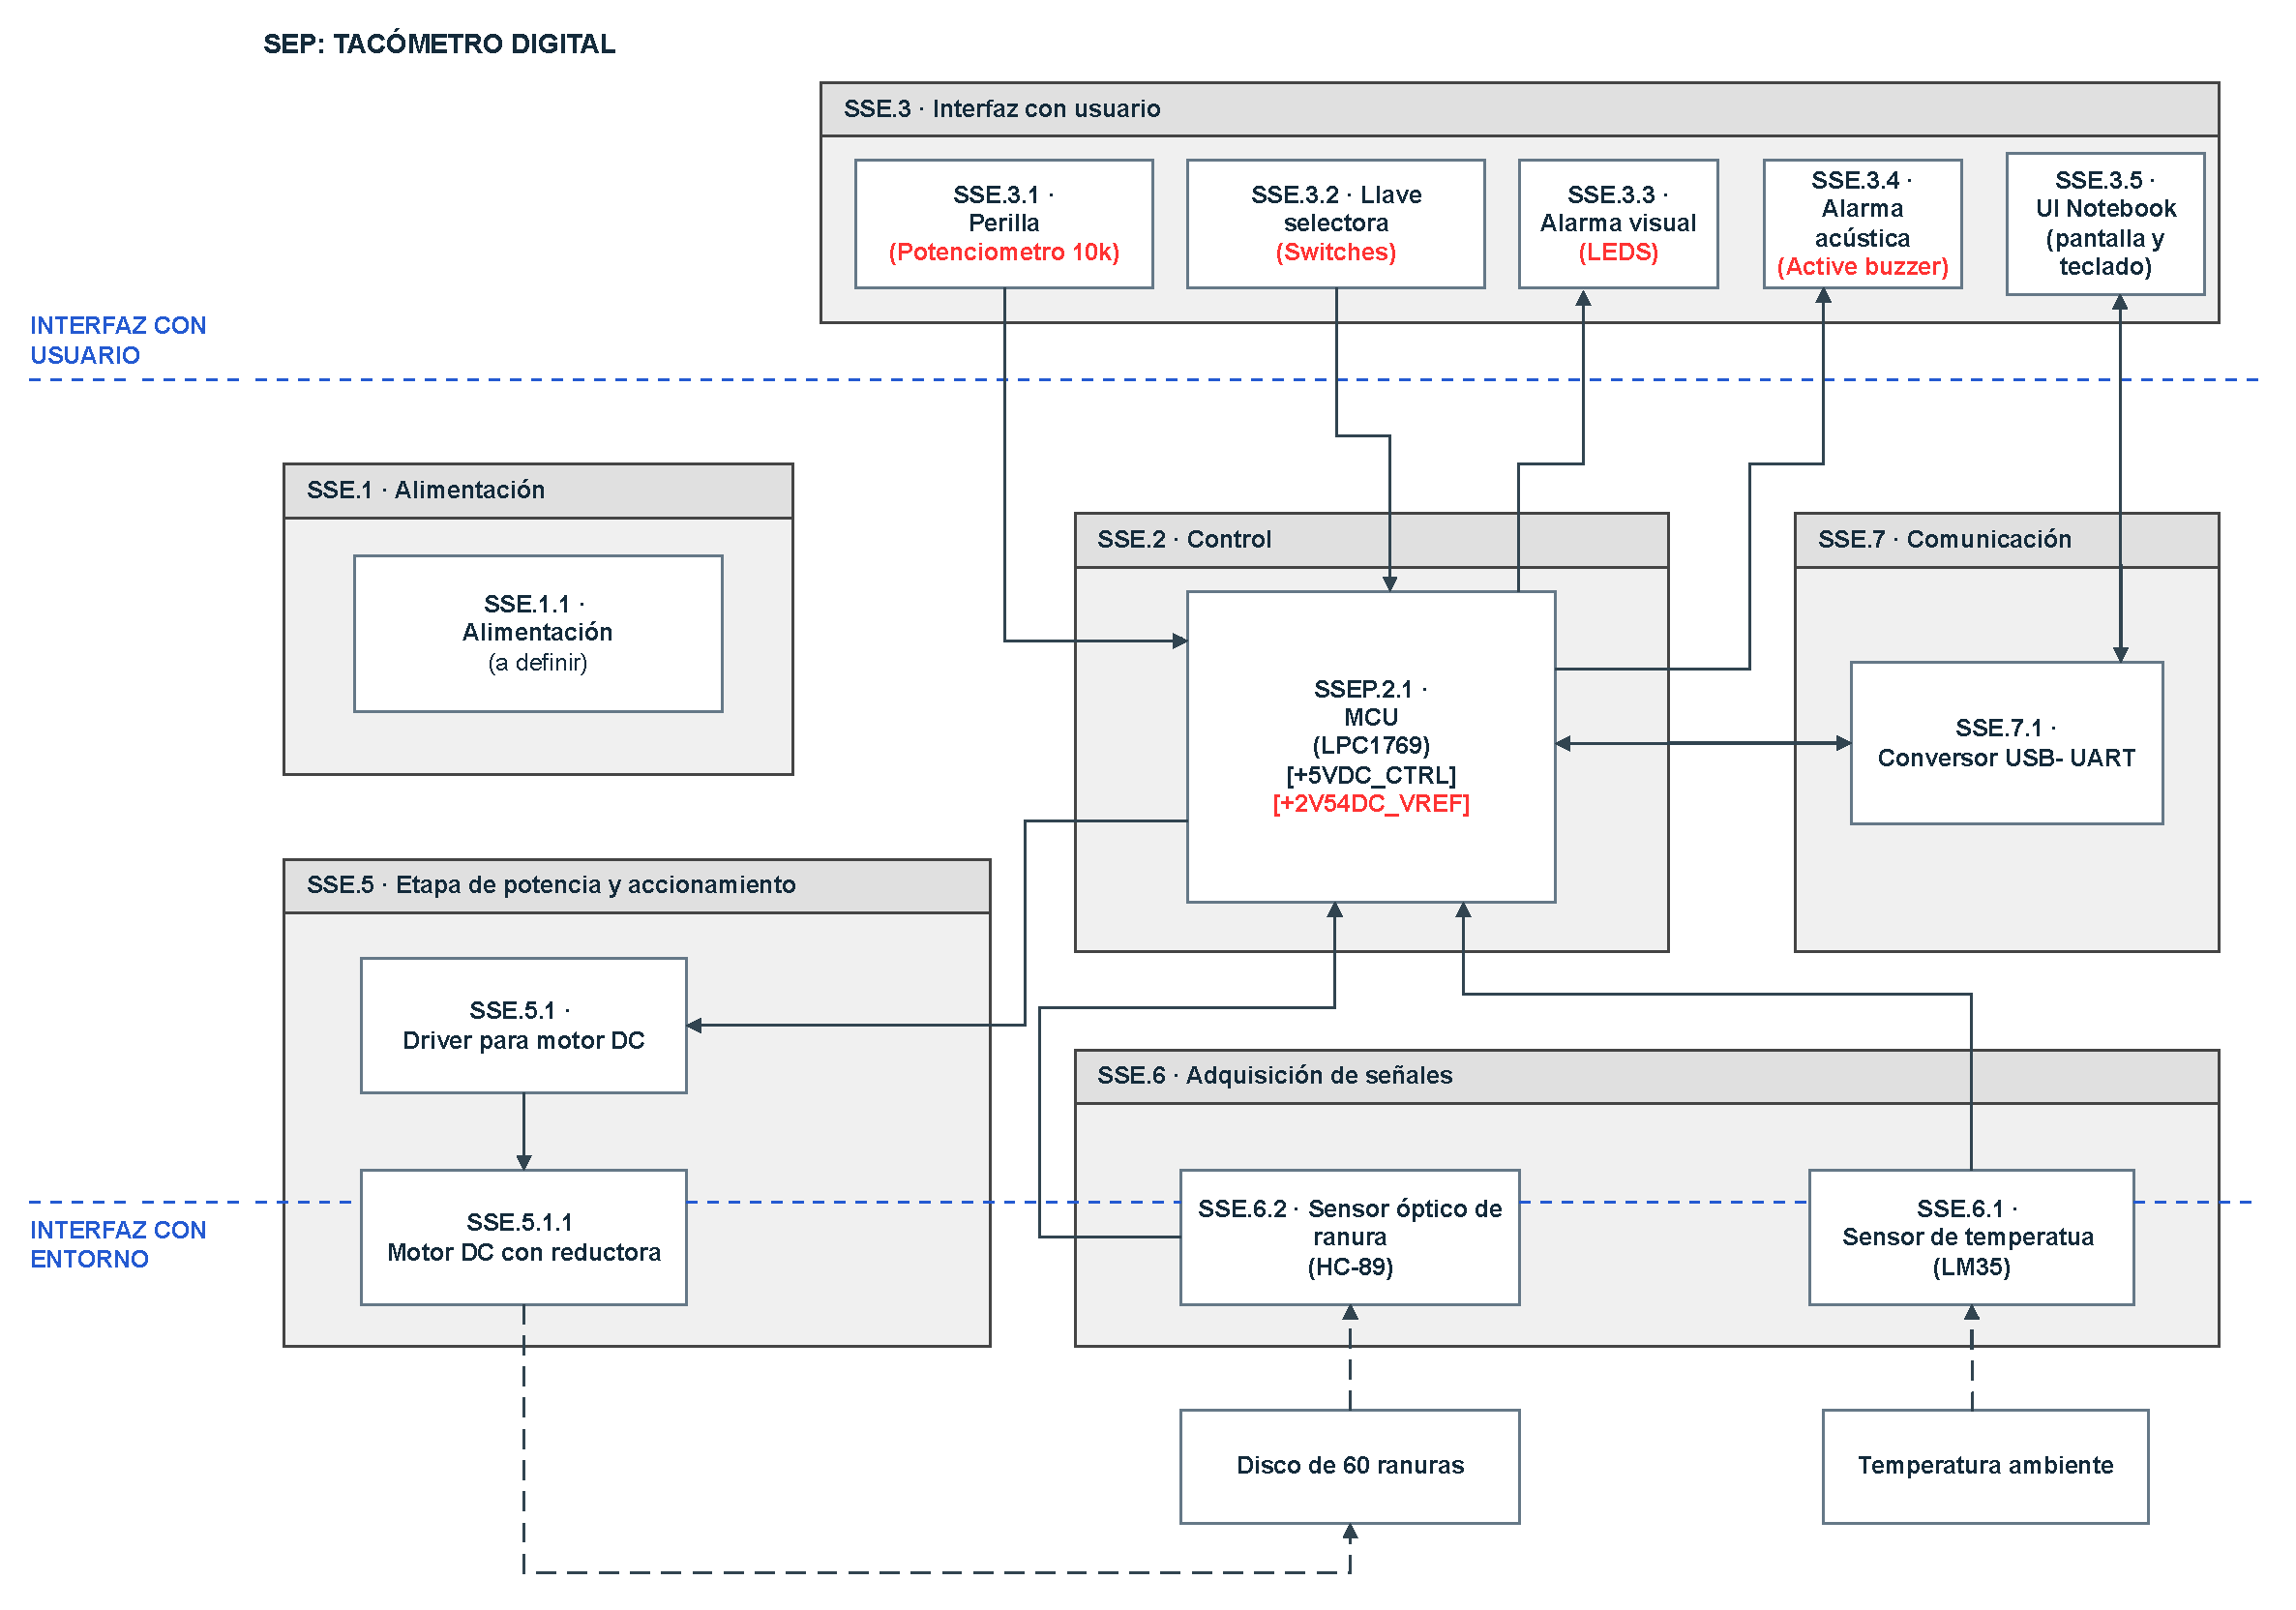
\includegraphics[width=\textwidth,height=0.75\textheight,keepaspectratio]{diagramas/hardware.pdf}
\end{center}

\pendiente{volver a exportar hardware.pdf desde hardware.drawio (ya actualizado con
XD-51 y VREFP 3,3\,V; falta completar la alimentación)}.

\clearpage
\subsection{ANEXO B: FIRMWARE DEL SEP}

\begin{center}
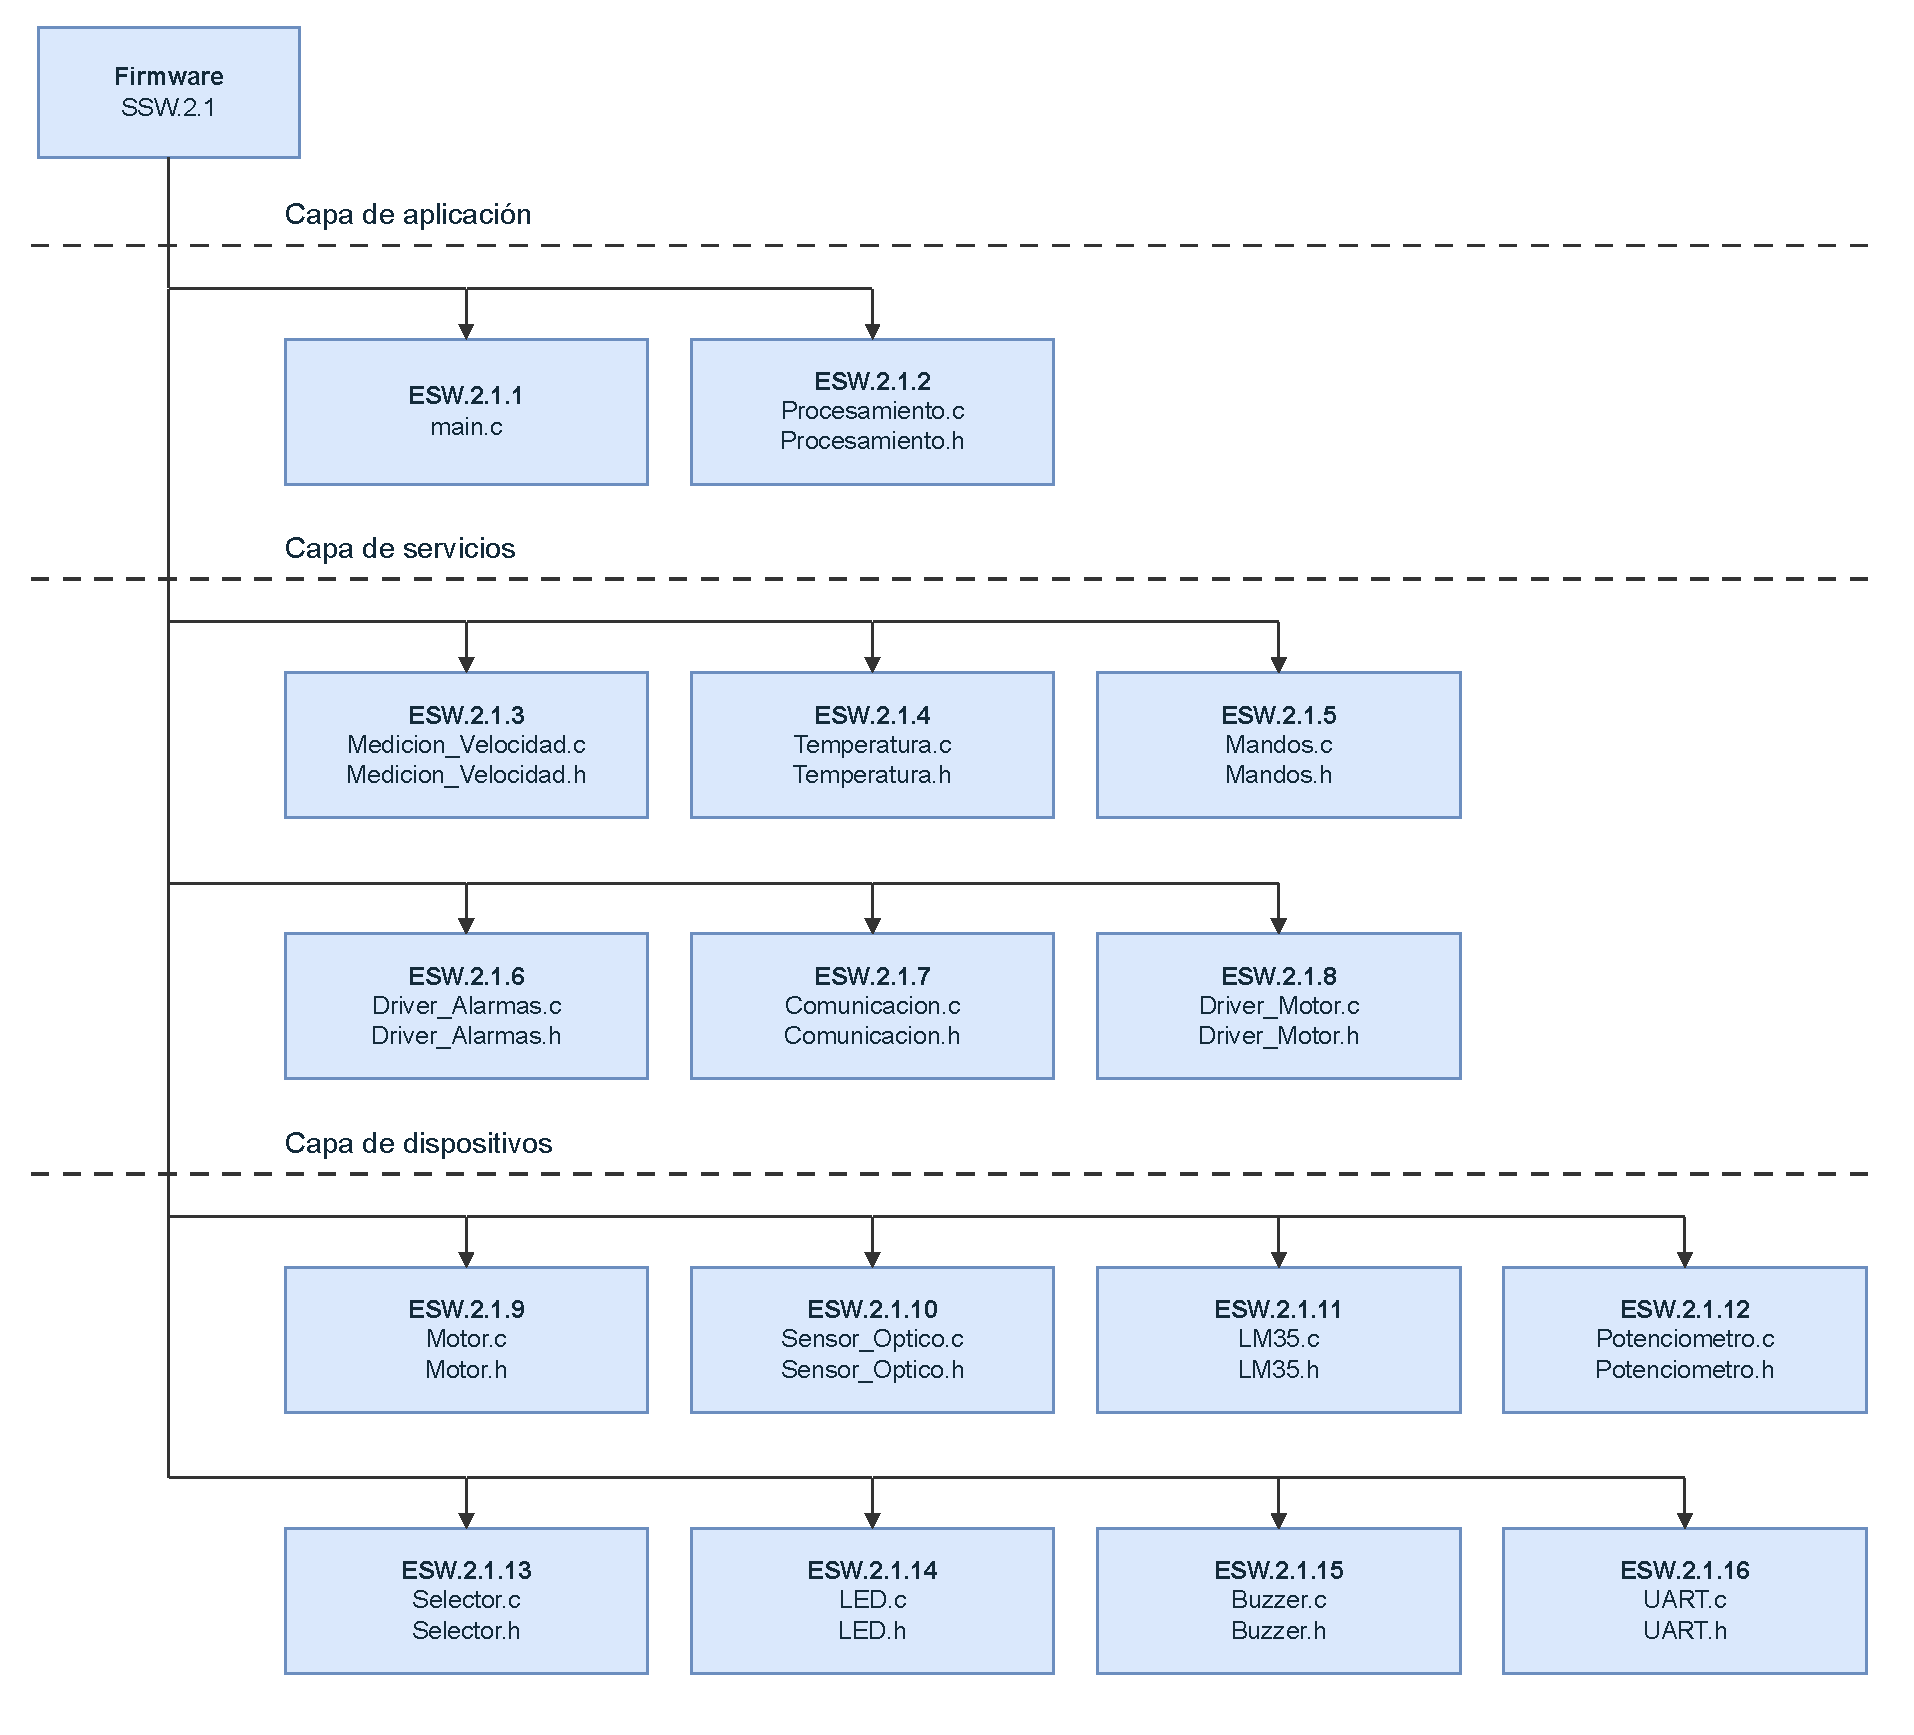
\includegraphics[width=\textwidth,height=0.75\textheight,keepaspectratio]{diagramas/firmware.pdf}
\end{center}

Los módulos de soporte de plataforma (Sistema, Reloj y Adquisicion\_ADC\_DMA), sin ESW
propio, se indican con borde punteado.
\pendiente{volver a exportar firmware.pdf desde firmware.drawio (ya actualizado con
ESW.2.1.17 y el soporte de plataforma)}.

\subsubsection{SECUENCIA DEL PERÍODO DE CONTROL}

La siguiente secuencia muestra cómo cooperan las capas en cada período de 500\,ms, en
modo automático con consigna activa:

\begin{enumerate}
  \item \texttt{TIMER0\_IRQHandler} (dispositivos) cierra la ventana: lee
  \texttt{SensorOptico\_Read} y publica los pulsos.
  \item \texttt{Aplicacion\_Iterar} llama a \texttt{Medicion\_Velocidad\_Actualizar}
  (servicios), que obtiene los pulsos con \texttt{Timer\_ConsumirVentana} y devuelve la
  velocidad en milésimas de RPM.
  \item \texttt{Aplicacion\_Periodo} llama a \texttt{Temperatura\_Leer} $\rightarrow$
  \texttt{LM35\_Read}; la decisión de \texttt{Procesamiento\_EvaluarAlarma} se aplica con
  \texttt{Driver\_Alarmas\_Aplicar} $\rightarrow$ \texttt{LED\_Write} y
  \texttt{Buzzer\_Write}.
  \item Lee las consignas con \texttt{Comunicacion\_RecibirConsigna} $\rightarrow$
  \texttt{UART\_Read} y la llave con \texttt{Mandos\_LeerModo} $\rightarrow$
  \texttt{Selector\_Read}; \texttt{Procesamiento\_ActualizarModo} devuelve el estado.
  \item \texttt{Procesamiento\_Regular} calcula el mando, que se aplica con
  \texttt{Driver\_Motor\_Aplicar} $\rightarrow$ \texttt{Motor\_Write}.
  \item \texttt{Comunicacion\_EnviarTelemetria} arma la trama y la encola con
  \texttt{UART\_Write}; \texttt{UART3\_IRQHandler} la transmite en segundo plano.
\end{enumerate}

\subsection{ANEXO C: CÓDIGO FUENTE}

El código fuente completo, documentado con Doxygen, se entrega en la carpeta
\texttt{Firmware/} y está disponible en el repositorio del proyecto.

\end{document}
